% вторая часть

\section{Проектирование и разработка приложения для задания параметров}

\subsection{Разработка вспомогательных классов}

Первоначальным этапом разработки было создание вспомогательных классов для работы с исходными данными.

Некоторые операции, которые являются общими для нескольких классов, могут быть перенесены на вспомогательные классы, которые затем используются с помощью композиции объекта. 

Каждый отдельный класс относится к конкретному типу файла. Для всех файлов мы можем выделить один общий метод – это чтение информации из файла. Чтобы не повторять в каждом классе эту операцию, можно воспользоваться одним из ключевых понятий объекто-ориентированного программирования, а именно – наследованием. 

Наследование является неотъемлемой частью Java. При использовании наследования вы говорите: этот новый класс похож на тот старый класс. В коде это пишется как extends, после которого указываете имя базового класса. Тем самым вы получаете доступ ко всем полям и методам базового класса. Используя наследование, можно создать общий класс, которые определяет характеристики, общие для набора связанных элементов. Затем вы можете наследоваться от него и создать новый класс, который будет иметь свои уникальные характеристики. Главный наследуемый класс в Java называют суперклассом. Наследующий класс называют подклассом. Получается, что подкласс — это специализированная версия суперкласса, которая наследует все члены суперкласса и добавляет свои собственные уникальные элементы.

Исходный код суперкласса приведён в приложении в листинге~\ref{DefReader}.

От этого суперкласса были наследованы все остальные подклассы, которые реализуют работу с каждым типом файлов. 

В основном, эти подклассы включают в себя методы, которые проводят синтаксический анализ (парсинг) полученного ранее текста файла. Затем, полученная в результате этой операции информация присваивается полям класса. Таким образом, текст файла структурируется по полям класса. 

Для корректного парсинга и выделения подстрок в программе использовались регулярные выражения. Функция setChans (листинг~\ref{list-1}) является примером реализации метода синтаксического анализа текста. 

\begin{Program}
	\begin{MyCode}
		private void setChans(){
			if (fileInf == null) {
				System.out.println("Error");
			} else {
				
				
				for (int i = 1; i <= n*2; i++) {
					String[] split = fileInf.get(i).trim().split("\\s+");
					if((split.length == 2) && (Integer.valueOf(split[1]) == 1)) {
						
						String[] split1 = fileInf.get(i+1).trim().split("\\s+");
						ChanProf ch = new ChanProf(Integer.valueOf(split[0]), Integer.valueOf(split1[0]), Integer.valueOf(split1[1]), split1[2]);
						chans.add(ch);
						
					}
					i++;
					
				}
			}
		}
			
		\end{MyCode}
		\caption{Обработка и синтаксический анализ текста}\label{list-1}
	\end{Program}


При анализе текста исходных файлов можно заметить, что в некоторых файлах имеются повторяющиеся строки с одинаковой структурой. Целесообразно выделить их в отдельные классы. Такие классы представляют собой структуры для хранения информации. Основные методы таких классов – это set- и get-методы.

Также, в отдельную группы можно выделить классы, которые работают с файлами, которые используются для сохранения результатов моделирования определенного канала. Структура таких фалов может меняться: некоторые столбцы могут добавляться или наоборот убраться. Поэтому, было решено выделить структуру этих файлов в отдельный файл с метаданными по столбцам. 

Пример такого файла представлен на рисунке~\ref{fig:meta}.
\begin{figure}[H]
	\centering
	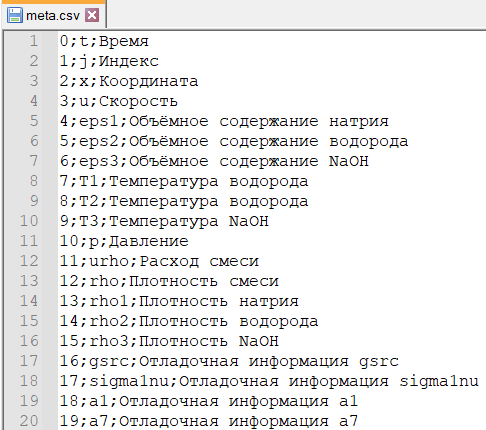
\includegraphics[width=0.7\linewidth]{pics/meta}
	\caption{Структура файла CSV}
	\label{fig:meta}
\end{figure}

Он представляет собой CSV-файл. В качестве разделителя здесь выступает точка с запятой. Первый столбец – это индекс столбца в файле с результатами моделирования канала. Второй столбец – это идентификатор переменной, который используется в выходном файле канала. Третий столбец – это полное название переменной. Оно нужно для последующего отображения в программе, чтобы пользователь мог выбрать конкретные физическое величины, а не идентификаторы. 

Для работы с файлом SCV и файлом с результатами моделирования канала было написано три класса: ChanCol, ChanFile и ChanInTime.

Класс ChanCol реализует колонку выходного файла с результатами. Поля этого класса полностью совпадают со структурой файла CSV. 

Исключение составляет лишь поле, в котором записан путь к файлу с данными по умолчанию. Так как CSV файла с метаданными по столбцам может попросту не быть, то было решено «вшить» в программу файл по умолчанию, в котором записана информация по колонкам, которая актуальна на данный момент. 

Также, момент с отсутствием файла с метаданными был учтён и в коде программы (листинг~\ref{list-2}).

\begin{Program}
	\begin{MyCode}
		try {
			br = new BufferedReader(new FileReader(path));
			while ((line = br.readLine()) != null) {
				String[] data = line.split(";");
				ChanCol chanCol = new ChanCol(Integer.valueOf(data[0]), data[1], data[2]);
				arr.add(chanCol);
				
			}
			
			
		} catch (FileNotFoundException ex) {
						
			try {
				br = new BufferedReader(new FileReader(ChanCol.defaultCSV));
				while ((line = br.readLine()) != null) {
					String[] data = line.split(";");
					ChanCol chanCol = new ChanCol(Integer.valueOf(data[0]), data[1], data[2]);
					arr.add(chanCol);
					
				}
				
			} catch (FileNotFoundException ex1) {
				Logger.getLogger(ChanCol.class.getName()).log(Level.SEVERE, null, ex1);
			} catch (IOException ex1) {
				Logger.getLogger(ChanCol.class.getName()).log(Level.SEVERE, null, ex1);
			}
		
	\end{MyCode}
	\caption{Обработка FileNotFoundException}\label{list-2}
\end{Program}

В вышеприведенном участке кода реализуется парсинг данных из файла CSV. В блоке catch (FileNotFoundException ex) производится обработка исключения FileNotFoundException. Если файл не найден, то для дальнейшей работы используется файл по умолчанию, упомянутый выше. 

Класс ChanInTime представляет состояния канала в заданный момент времени. В качестве полей класса выступают такие значения, как время, список переменных (массив объектов класса ChanCol) и список массивов значений столбцов. Объект такого класса представляет собой строки выходного файла, которые соответствуют заданному моменту времени. Т.е. мы имеем один момент времени и несколько точек, которым соответствуют значения из файла с результатами моделирования.

Класс ChanFile представляет данные из расчетного файла в виде массива (списка) состояний в каждый момент времени. Здесь используется описанный выше класс ChanInTime. Массив из объектов этого класса будет описывать все моменты времени моделирования. Таким образом, объект класса ChanFile будет содержать в себе полную информацию выходного файла с результатами моделирования.

\subsection{Разработка пользовательского интерфейса}

Приложение представляет собой программу, написанную на языке Java с использованием технологии Swing. Графический интерфейс позволяет удобно и интуитивно работать с программой. Приложение облегчает работу пользователя, т.к. проводит выборку необходимых параметров для визуализации автоматически. 
Программа представляет собой приложение с графическим интерфейсом, состоящее из нескольких окон: начальное окно с выбором директории, в которой содержатся исходные файлы, главное меню и окна с выбором параметров. 

\subsubsection{Окно выбора директории}

При запуске программы первое окно, которое видит пользователь – это окно выбора директории с исходными файлами (рисунок~\ref{fig:dir}). 
\begin{figure}[H]
	\centering
	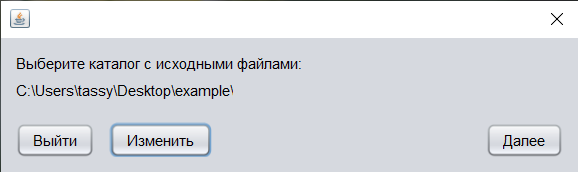
\includegraphics[width=0.7\linewidth]{pics/dir}
	\caption{Окно выбора директории}
	\label{fig:dir}
\end{figure}

В окне представлены три кнопки: «Выйти», «Изменить» и «Далее». 

При нажатии на кнопку «Изменить», открывается диалоговое окно с выбором каталога (рисунок~\ref{fig:edit-dir}).
\begin{figure}[H]
	\centering
	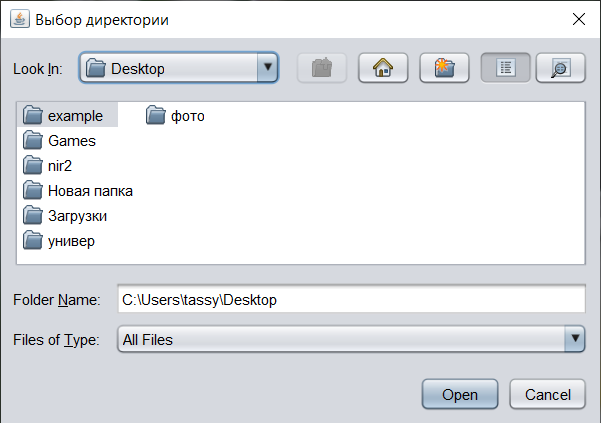
\includegraphics[width=0.7\linewidth]{pics/edit-dir}
	\caption{Диалоговое окно изменения директории}
	\label{fig:edit-dir}
\end{figure}

Указание директории при начале работы необходимо для корректной работы программы. Приложение использует данные из исходных файлов для отображения в пользовательском интерфейсе. В программе также предусмотрена возможность смены директории исходных файлов из главного меню.


\subsubsection{Главное меню}

После выбора исходной директории, при нажатии кнопки «Далее» происходит переход к окну с главным меню. 
\begin{figure}[H]
	\centering
	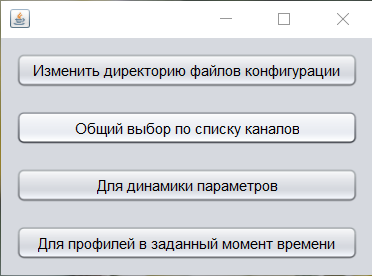
\includegraphics[width=0.7\linewidth]{pics/menu}
	\caption{Главное меню}
	\label{fig:menu}
\end{figure}

В главном меню собраны кнопки, отвечающие за основной функционал программы (рисунок~\ref{fig:menu}). Здесь присутствует кнопка «Изменить директорию файлов конфигурации». По своему функционалу она схожу с начальным окном выбора каталога. После неё идет группа из трёх кнопок, которые отвечают за задание параметров расчетных данных. В эту группу входят: выбор по списку каналов, выбор для динамики параметров и выбор для профилей в заданный момент времени. 

\subsubsection{Общий выбор по списку каналов}

Данное окно вызывается из окна с главным меню. В нём предоставляется возможность выбора канала, для которого нужно проводить визуализацию (рисунок~\ref{fig:chan}).
\begin{figure}[H]
	\centering
	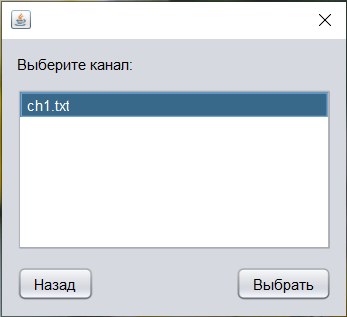
\includegraphics[width=0.4\linewidth]{pics/chan}
	\caption{Окно общего выбора по списку каналов}
	\label{fig:chan}
\end{figure}

В окне есть две кнопки: «Назад» и «Выбрать». Каналы выводятся в JList. JList используются для визуального отображения данных.  Выборка данных производится из файла, который содержит информацию о каналах (chanprof.txt). Загрузка и обработка данных совершается с помощью класса ChanProfReader. Он выполняет считывание и парсинг необходимых данных из файла конфигурации. 


\subsubsection{Выбор для динамики параметров}
Данное окно вызывается из окна с главным меню. В нём предоставляется возможность выбора координаты канала и переменных для отображения (рисунок~\ref{fig:dynam}).

\begin{figure}[H]
	\centering
	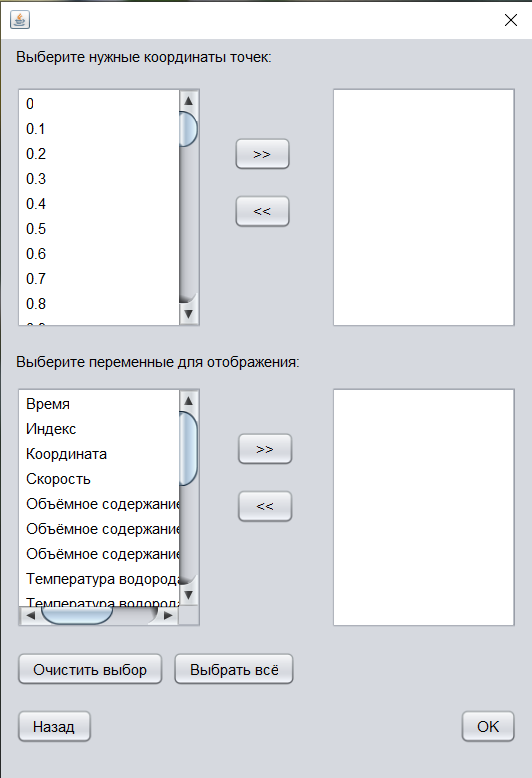
\includegraphics[width=0.5\linewidth]{pics/dynam}
	\caption{Окно выбора для динамики параметров}
	\label{fig:dynam}
\end{figure}

В окне представлены несколько списков, в которых отображаются доступные для выбора параметры и выбранные параметры (рисунок~\ref{fig:dynam-select}). Для осуществления выбора в окне есть несколько кнопок. Направление стрелок на кнопках соответствует направлению перемещения элементов из одного списка в другой. Также в окне присутствуют кнопки «Выбрать всё» и «Очистить список». Они реализуют упомянутые операции для элементов списка с параметрами наблюдений (рисунок~\ref{fig:dynam-all}). 
\begin{figure}[H]
	\centering
	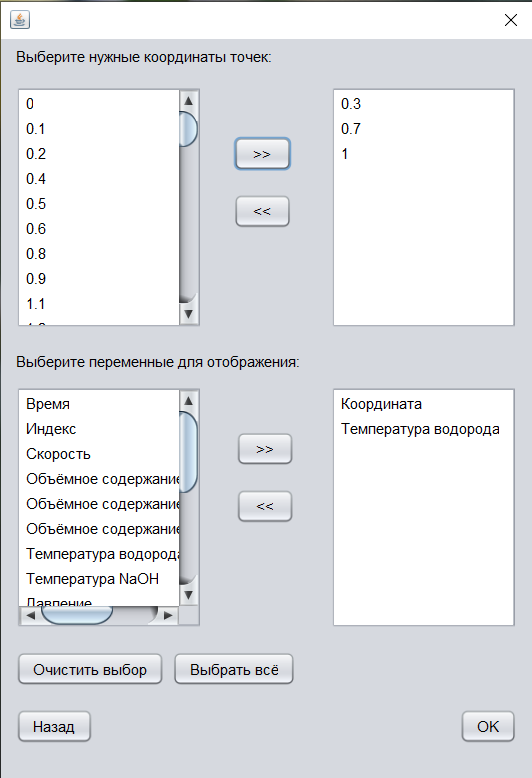
\includegraphics[width=0.5\linewidth]{pics/dynam-select}
	\caption{Окно выбора для динамики параметров}
	\label{fig:dynam-select}
\end{figure}

\begin{figure}[H]
	\centering
	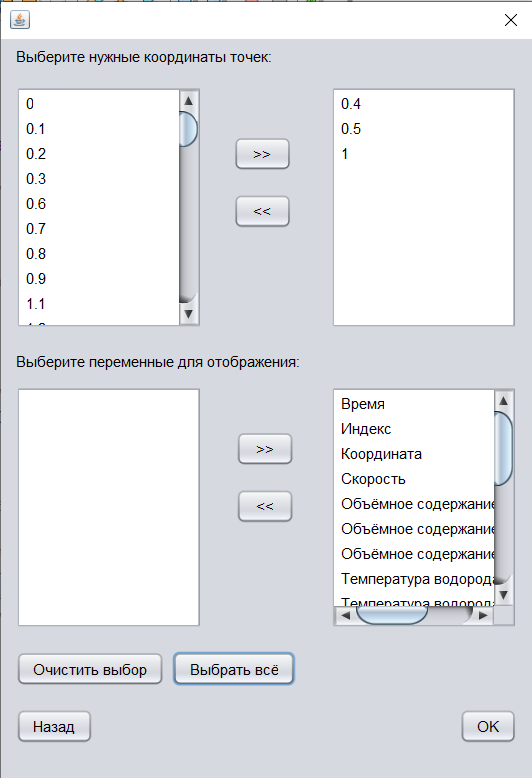
\includegraphics[width=0.5\linewidth]{pics/dynam-all}
	\caption{Окно выбора для динамики параметров}
	\label{fig:dynam-all}
\end{figure}

Выборка координат канала производится из файла с геометрий канала (geom.txt). Для этого производится подсчёт допустимых координат: исходя из шага сетки и длины канала, в цикле высчитываются все возможные координаты канала. Весь описанный функционал выполняется через класс GeomReader, который реализует считывание данных и их последующую обработку и необходимые вычисления. 

Выборка переменных для отображения производится из CSV-файла с метаданными по параметрам. Выполняется это с помощью класса CSVReader, который реализует считывание данных и их последующую обработку.

\subsubsection{Выбор для профилей в заданный момент времени}

Данное окно вызывается из окна с главным меню. В нём предоставляется возможность выбора момента времени моделирования и переменных для отображения (рисунок~\ref{fig:time}).

\begin{figure}[H]
	\centering
	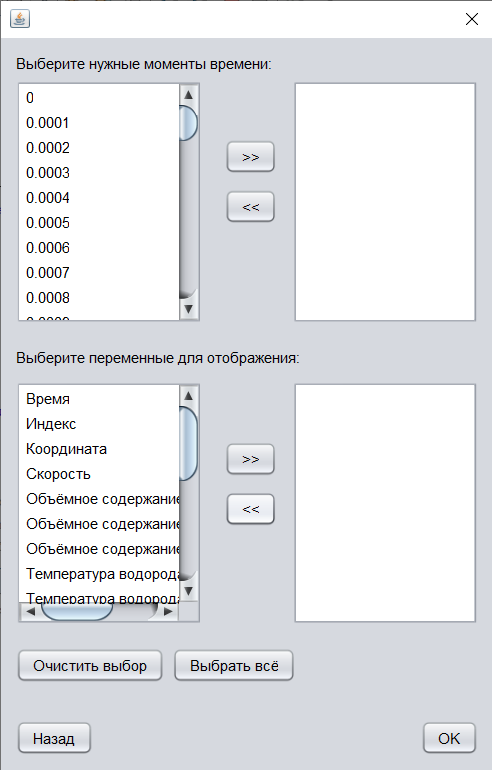
\includegraphics[width=0.5\linewidth]{pics/time}
	\caption{Окно выбора для профилей в заданный момент времени}
	\label{fig:time}
\end{figure}

В окне представлены несколько списков, в которых отображаются доступные для выбора параметры и выбранные параметры (рисунок~\ref{fig:time-select}). Для осуществления выбора в окне есть несколько кнопок. Направление стрелок на кнопках соответствует направлению перемещения элементов из одного списка в другой. Также в окне присутствуют кнопки «Выбрать всё» и «Очистить список». Они реализуют упомянутые операции для элементов списка с параметрами наблюдений (рисунок~\ref{fig:time-all}). 

\begin{figure}[H]
	\centering
	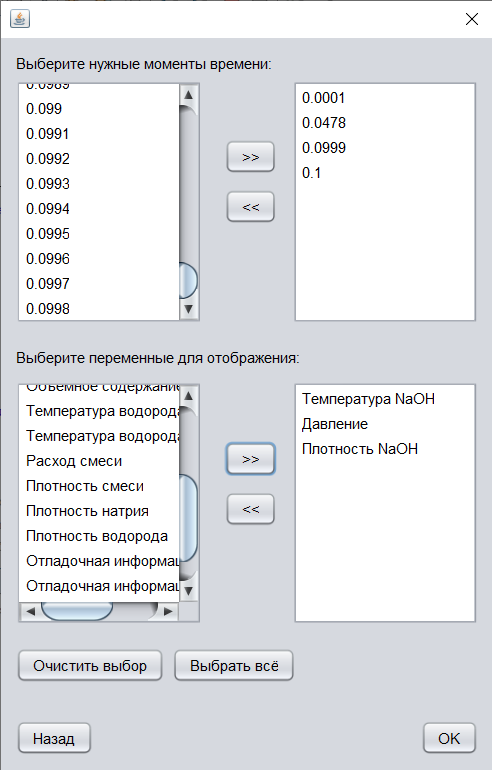
\includegraphics[width=0.5\linewidth]{pics/time-select}
	\caption{Окно выбора для профилей в заданный момент времени}
	\label{fig:time-select}
\end{figure}

\begin{figure}[H]
	\centering
	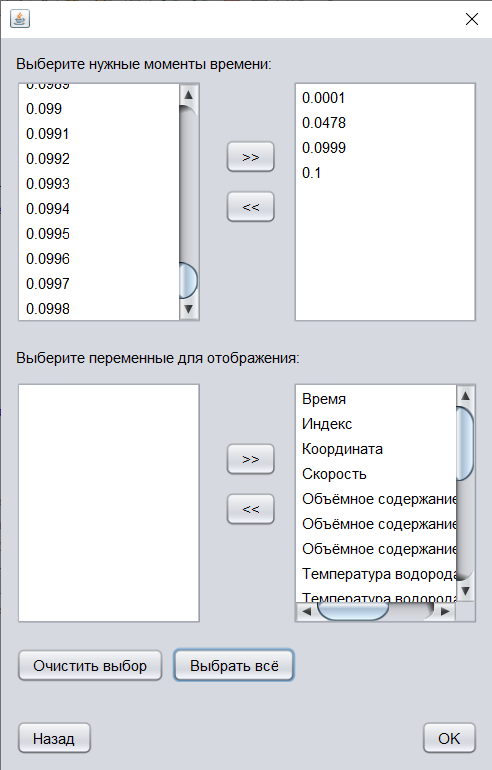
\includegraphics[width=0.5\linewidth]{pics/time-all}
	\caption{Окно выбора для профилей в заданный момент времени}
	\label{fig:time-all}
\end{figure}
Выборка моментов времени производится из файла со сценарием сохранения результатов (timescen.txt). Для этого производится подсчёт допустимых моментов времени: исходя из количества временных интервалов моделирования и шага интервалов, в цикле высчитываются все возможные временные моменты. Весь описанный функционал выполняется через класс TimeReader, который реализует считывание данных и их последующую обработку и необходимые вычисления. 

Выборка переменных для отображения производится так же, как и в окне выбора для динамики параметров. 

